\documentclass[]{article}
\usepackage[nodayofweek,level]{datetime}
\usepackage{hyperref}
\usepackage{listings}
\usepackage{centernot}
\usepackage{amsmath,amssymb}
\usepackage{graphicx}
\usepackage{filecontents}
\newcommand{\rithm}{\textbf{RiTHM}\space}
\newcommand{\tloss}{\emph{transient loss of trace}}
\newcommand{\ploss}{\emph{persistent loss of trace}}

% Title Page
\title{\rithm development status report}
\author{}


\begin{document}
\maketitle


\begin{abstract}
Details about the current progress of \rithm development and journal paper
\end{abstract}
\section{Current Results and Details about on-going items}

			\subsection{Runtime verification in case of Missing Events}
			Important sections for the paper to be submitted are proposed as per below

			\subsubsection{Introduction}
			\begin{itemize}
				\item LTL as industry standard for verification; LTL on finite paths
				\item Berief description of problem of \emph{runtime verification} in the event of loss of trace, and practical scenarios; Considerations w.r.t. \emph{reactive systems},  \emph{instrumentation overhead}, \emph{monitoring overhead}.
				\item Brief description of previous work on \emph{monitoring} in case of loss of trace; Consideration of contributions by Smolka et al. and related papers (to be surveyed)
				\item Benefits and limitations of previous work.
				\item Description of our approach of problem solving; Extending the definition of monitorability provided by Falcone et al. in \cite{RefWorks:9} in the event of loss of \emph{trace}; Extending definition of \emph{soundess} by building upon the current definition which describes \emph{soundess} as absence of \emph{false negatives};	Description of \ploss{} and \tloss
				\item Brief description of the decision procedure to identify \emph{monitorable} formulae from \emph{LTL hierarchy} in \cite{RefWorks:11}  when there is a \tloss; Details of another decision procedure to monitor LTL formulae at runtime depending upon the state of the monitor.
				\item Brief description of \emph{proof} of correctness of monitoring for both decision procedures
				\item Benefits of our approaches w.r.t.  \emph{deadlines in reactive systems},  \emph{reduced instrumentation overhead}, \emph {reduced monitoring overhead}.
			\end{itemize}
			
			\subsubsection{Background}
			\begin{itemize}
				\item Definition of \tloss{} and \ploss{} in context of \emph{Reactive Systems}; Practical scenarios and examples. (Survey to be done for citing examples in real world)
				\item Formal Definitions of \tloss{} and \ploss{} in context of \emph{Runtime Verification}; Builiding up on the notion of \emph{finite/persistent} loss of stream of alphabets.
				\item Overview of \emph{Runtime Verification}
				\item Details of LTL - definition, semantics; Overview of LTL hierarchy by Pnueli et al. in \cite{RefWorks:11}
				\item Background on LTL on finite paths - 3-valued semantics by Leucker et al. in \cite{RefWorks:10}; 4-valued semantics by Bauer et al. in \cite{RefWorks:12}; Method to generate monitors described in \cite{RefWorks:10}.
				\item Definition of monitorability by Falcone et al. in \cite{RefWorks:9} which builds up on classes of LTL - \emph{Prefix Properties}, \emph{Recurrence - b\"{u}chi} and \emph{Persistence - co-b\"{u}chi} properties. Highlighting the monitoring definition of \emph{Recurrence - b\"{u}chi} and \emph{Persistence - co-b\"{u}chi} properties by Falcone et al.
				\item Extension of 4-valued semantics by Schneider et al. in \cite{RefWorks:17}.
			\end{itemize}
			
			\subsubsection{Related Work}
			\begin{itemize}
				\item Contributions by Smolka et al. in \cite{RefWorks:14} and the benefits and limitations of their approach. Emphasis on the limitations of the method to arrive at probabilities.
				\item Our approach and the \emph{stringent} notion of \emph{soundness} for our decision procedures as compared to the one proposed in \cite{RefWorks:14} by Smolka et al.
				\item Survey to be done on other papers.
			\end{itemize}
			
			\subsubsection{Our Approach}
				\begin{itemize}
					\item We describe the first part of the problem as "Which LTL formulae are \emph{monitorable} in the event of \tloss{} and subsequent \emph{guaranteed} recovery of the system from the loss?"
					\item Description of the decision procedure to generate LTL$_4$ monitor using the method described in \cite{RefWorks:10}
					\item Describe our algorithm which asserts whether a LTL specification is \emph{monitorable} in the event of \tloss{}; We build up the algorithm on the notion of absence of states in the FSM which are labelled as $\top$ or $\bot$ and all transitions to states in the FSM which are marked as $\top_p$ and $\bot_p$  are unique for different possible conjunctions of predicate symbols or their negations i.e. each alphabet of a finite / infinite word causes transition to a unique state for the given FSM.
					\item Practical examples of such specifications - \emph{Recurrence} and \emph{Persistence} class.
					\item Definition of \emph{Soundness} in the event of \tloss{}; We build up the definition on the notion that if the system recovers from a \tloss{}, the truth value of the monitor never allows \emph{false-negatives}.
					\item Proof of correctness of the decision procedure w.r.t new defintion of \emph{Soundness}; We build up the proof from the details top of classes of LTL hierarchy and our criteria w.r.t. the restrictions on the LTL$_4$ monitor. Proof includes consideration of infinite path.
					\item Description of second problem. A superset of the class of specifications which can be monitored in the event of \tloss{}, is described. The formulae in this superset could be monitored at runtime depending on the state of LTL$_4$ monitor.
					\item Proof of correctness for the second decision procedure and examples of the associated specifications
					
				\end{itemize}
			\subsubsection{Empirical Evaluation}	
				\begin{itemize}
					\item Examples of monitoring incomplete data w.r.t the second decision procedure.
					\item Details of examples where the instrumentation is performed by DIME.
				\end{itemize}
	\subsection{\rithm development work}
	\begin{itemize}
	\item MTL parser has been developed, the monitor for MTL is being developed. \textbf{Update}: Including both Past-time and future-time MTL variants. 
	\item For developing predicate specification language, work is done on analysis of script engines which can be used. Beanshell \url{http://www.beanshell.org/intro.html} is under consideration along with JavaScript engines which can be embedded into java code, and the predicate definitions could be specified using the languages of these engines.
	
	\item IronForge data, and running \rithm on the properties of the data. Work in Progress.
	
	\item Integration of DIME + \rithm - Papers worked on for analyzing the previous work. Work done by Smolka et al. focuses on using Markov Chains for providing probabilistic estimates on the satisfaction of specifications. On similar lines, Probabilistic Timed Automata could be used for specifying 
	models of systems which exhibit the characteristics of incomplete-data for verification along with the requirement of hard real-time deadlines.
	\item 'Lessons Learnt' section for journal paper is being worked upon.
	
	\item \rithm's monitor using specifications in the format of regular expressions is being enhanced so that monitoring is trace-length independent. The coding is in progress and we now use \url{http://www.brics.dk/automaton/doc/index.html} to create automaton from regular expression and input trace ti this automaton event by event. 
	

	

	\end{itemize}
	
\section{Previous Results}

		\subsection{Runtime verification in case of Missing Events}
		\textbf{Updates on \formatdate{7}{4} {2015}}\newline
		\begin{itemize}
			
			\item \textbf{Missing Events} correspond to the case when Runtime Monitor does not receive a trace from the program which is being monitored.
			
			\item Events could be missed for a \emph{finite} amount of time or there could be \emph{persistent}. This loss of a stream of events could be formalized as either a \emph{finite} path within the program when the events could not be monitored or a possible \emph{infinite} path within the program when the events could not be monitored.
			
			\item In case of loss of trace for \emph{finite} time, the monitor cannot keep track of a finite path which is being executed in the program and hence it cannot provide verdict of certain type of \emph{LTL} properties.
			
			\item On the other hand, a \emph{persistent} loss of program trace implies that the monitor cannot validate any type of \emph{LTL} property.
			
			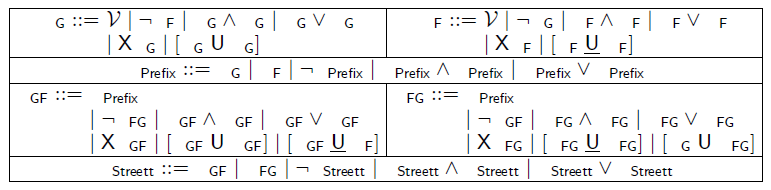
\includegraphics[scale=0.4]{LTLHierarchy.png}
			
			\item In above, \emph{LTL} hierarchy, there are 6 classes of specifications and the class \emph{Street} is the most expressive one and for most of the LTL formulae, it is not difficult to find an equivalent class which belongs to the class \emph{Street}.
			
			\item Among the classes in \emph{LTL} hierarchy, in the event of loss of trace for a \emph{finite} path within the program, it is not possible to preserve soundness while monitoring \emph{Safety $(P_G)$}, \emph{Liveness $(P_F)$} and \emph{Prefix} which is boolean closure of \emph{Safety} and \emph{Liveness}
			
			\item This happens because a \emph{Liveness} property could be satisfied by a \emph{finite} path of a \emph{reactive} system and a \emph{Safety} property could be violated by \emph{finite} path. This \emph{finite} path could be the path whose trace was lost. Hence, the verdict given by a \emph{LTL} monitor might not show the actual status.
			
			\item On the other hand, the properties in the class \emph{Recurrence ($P_{GF}$)} and \emph{Persistence ($P_{FG}$)} could be monitored by tolerating a loss of trace for a \emph{finite} path in the program provided certain criteria are fulfilled by states of \emph{LTL} monitor.
			
			\item The formulas which belong to the class \emph{Recurrence ($P_{GF}$)} have B\"{u}chi acceptance condition where one of the final states if the B\"{u}chi automaton should visited by the run of infinite word infinitely often. Hence, a \emph{finite} loss of program trace would not affect the monitoring provided the monitor (which is constructed from B\"{u}chi automaton) visits one of the final states infinitely often.
			
			\item The formulas which belong to the class \emph{Persistence ($P_{FG}$)} have Persistence acceptance condition where one of the final states if the Persistence automaton should be continuously visited by the run of infinite word. Hence, a \emph{finite} loss of program trace would not affect the monitoring provided the monitor eventually visits one of the final states in a continuous manner.
			
			\item \emph{Strett} class, which is boolean closure of \emph{Persistence} and \emph{Recurrence} classes exhibits a combination of acceptance conditions of \emph{Persistence} and \emph{Recurrence}. 	
			
			\item For example., below LTL$_4$ monitor belongs to the \emph{Persistence} property $\diamondsuit \square a$ U $b$. Here, provided the monitor is in one of the states among (0,1), (1,0), (1,1), a finite loss of a stream of events could be tolerated without violating the \emph{asymptotic} evaluation the truth value of the formula. 
			
			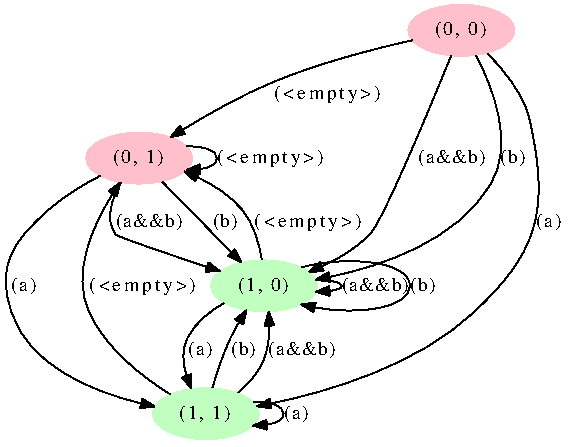
\includegraphics[scale=0.6]{FGExample.png}
			
			\item Below LTL$_4$ monitor belongs to the \emph{Recurrence} property $\square \diamondsuit  a$ U $b$. Here, provided the monitor is in one of the states among (0,1), (1,0), a finite loss of a stream of events could be tolerated without violating the \emph{asymptotic} evaluation the truth value of the formula. 
			
			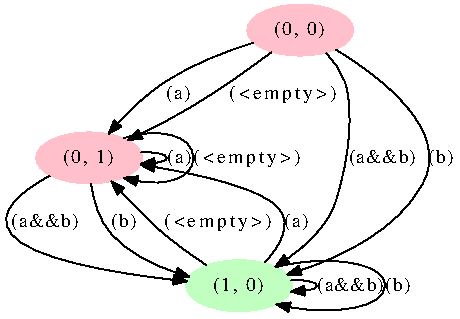
\includegraphics[scale=0.6]{GFExample.png}
			
			\item Future directions can include the proof of asymptotic correctness of the valuation of truth-value in the event of \emph{finite} loss of trace for  \emph{Recurrence ($P_{GF}$)}, \emph{Persistence ($P_{FG}$)} and \emph{Strett} classes.
			
		\end{itemize}
		
	\subsection{\rithm development and CRV'15 conference updates}
	\textbf{Updates on \formatdate{2}{4} {2015}}\newline
	\begin{itemize}

	\item
	\rithm For CRV'15 competition which will be held with RV'15 conference, benchmarks are submitted for 'C' program monitoring track and Offline Monitoring track.
	The details of benchmarks which are submitted can be found at 
	\begin{itemize}
		\item For 'C' program monitoring track - \url{https://forge.imag.fr/plugins/mediawiki/wiki/crv15/index.php/C_track}
		\item For Offline monitoring track \url{https://forge.imag.fr/plugins/mediawiki/wiki/crv15/index.php/Offline_track}
	\end{itemize}
	\item The 'C' program benchmarks are designed to monitor a 'C' program which launches 0.1 million POSIX threads, and various properties have been specified using First Order Linear Temporal Logic (Past as well as Future time)
	\item 'C' program which is being monitored can be found at \url{https://github.com/yogirjoshi/CRVBenchMark}
	\item The specifications for 'C' program monitoring track are as per below
	\begin{itemize}
		\item $\forall$ tid: pthread\_create(tid) $\longrightarrow$ $\diamondsuit$ pthread\_running(tid)
		\item $\forall$ tid: pthread\_mutex\_lock(tid, "ex\_mutex") $\longrightarrow$ $\diamondsuit$ pthread\_mutex\_unlock(tid, "ex\_mutex")
		\item $\forall$ tid: pthread\_create(tid) $\longrightarrow$ $\diamondsuit$ pthread\_join(tid)
		\item $\forall$ tid: (pthread\_mutex\_lock(tid, 'ex\_mutex') $\vee$ pthread\_mutex\_destroy(tid, 'ex\_mutex') $\vee$ pthread\_mutex\_unlock(tid, 'ex\_mutex')) $\longrightarrow$ $\diamondsuit^{-1}$ pthread\_mutex\_init(10000, 'ex\_mutex')))
		\item $\forall$ tid: (pthread\_exit(tid)) $\longrightarrow$ $\diamondsuit^{-1}$ pthread\_mutex\_unlock(tid, 'ex\_mutex'))
	\end{itemize}
	\item For offline monitoring track, QNX trace-logger files have been used. The trace file is at \url{https://github.com/yogirjoshi/datatools/blob/master/CRV1.tar.gz}. It contains 0.1 million events on which the specifications will be validated.
	\item Specifications are defined on various events of QNX threads. The specifications are as per below
	\begin{itemize}
		\item $\forall$  pid, $\forall$ tid : (thcreate $\longrightarrow$  $\diamondsuit$ thrunning)  (Satisfied by trace)
		\item $\forall$ $>90\%$ pid, $\forall$ tid : ($\diamondsuit$ threply) - Vioated by trace
		\item $\forall$  pid, $\forall$ tid : ($\square$ (thready $\longrightarrow$   $\diamondsuit$ thrunning)) - Satisfied by trace
		\item $\exists$ $=1$ pid, $\exists$ $=2$ tid: $\lnot$ ($\square$ ( $\lnot$ thdestroy)) - Vioated by trace
		\item $\forall$ $>50\%$ pid, $\forall$ $>50\%$ tid: ( $\diamondsuit$ ( thsem $\vee$ thmutex ) ) - Vioated by trace
	\end{itemize}
	
	\item
	\textbf{Updates on \formatdate{24}{3} {2015}}\newline
	Verbose LTL parser is implemented which uses verbose representation of LTL operators. \newline
	The code is at \url{https://github.com/yogirjoshi/parsertools.git}.
	
	\item
	Verbose LTL parser is integrated with existing LTL monitor. Some new APIs added to Parser interface for rewriting the specifications into interchangable formats. The code is at \url{https://github.com/yogirjoshi/monitortools.git}
	
	\item
	\rithm plugin loader is implemented so that different monitors, parsers and data-importers can be plugged in and used. \newline
	Below example starts \rithm instance to monitor LTL specifications using four valued semantics, and it uses CSV data
	
	\begin{lstlisting}
	java rithm.driver.RiTHMBrewer 
	-specFile=/home/y2joshi/InputFiles/specsQnx 
	-dataFile=/home/y2joshi/Input1.csv
	-outputFile=/home/y2joshi/InputFiles/output3.html 
	-monitorClass=LTL4 
	-traceParserClass=CSV 
	-specParserClass=LTL
	\end{lstlisting}
	Similarly, \rithm's another instance can be started to monitor using Verbose LTL (using 4-valued semantics), and it uses trace data in XML format 
	\begin{lstlisting}
	java rithm.driver.RiTHMBrewer 
	-specFile=/home/y2joshi/InputFiles/specsQnx 
	-dataFile=/home/y2joshi/Input1.XML
	-outputFile=/home/y2joshi/InputFiles/output3.html 
	-monitorClass=LTL4 
	-traceParserClass=CSV 
	-specParserClass=VLTL
	\end{lstlisting}
	\item \rithm can import data in CSV format and the CSV data-importer is intergrated with \rithm framework
	
	\item
	\rithm source has been refactored to use maven for project source code and build management. \rithm source has been enhanced to drop some legacy APIs to make the design more scalable
	
	\item API key feature for \rithm is being implemented. The API key will allow access management for \rithm when used in server mode.
	\end{itemize}

	\bibliographystyle{acm}
	\nocite{*}
	\bibliography{bibList}

	
\end{document}      
